\section{Izomerie a NMR}

\subsection{Izomerie}

Sloučeniny mají stejný sumární vzorec, ale rozdílnou strukturu.

\textbf{Konstituční (strukturní) izomery} se liší polohou jednotlivých atomů v molekule:
\begin{itemize}
	\item \textbf{Polohové izomery} se liší polohou funkční skupiny v molekule: 1-chlorpropan a 2-chlorpropan.
	\item \textbf{Funkční izomery} se liší typem funkční skupiny, např. ethanol a dimethylether.
	\item \textbf{Tautomery} se liší polohou vodíku a dvojné vazby, např. izomery acetylacetonu.
\end{itemize}

\textbf{Stereoizomery} se liší prostorovou geometrií:
\begin{itemize}
	\item \textbf{Cis--trans izomerie}
	\item \textbf{Konformery}
	\item \textbf{Enantiomery neboli optické izomery}, chirální látky lišící se rovinou stáčení polarizovaného světla
\end{itemize}

\subsection{NMR -- počet a intenzita signálů}

\begin{itemize}
	\item Stručně princip NMR, jaderný spin, supravodivé magnety
	\item Důležitá jádra, \ce{^1H}, \ce{^{13}C}, \ce{^{19}F}
\end{itemize}

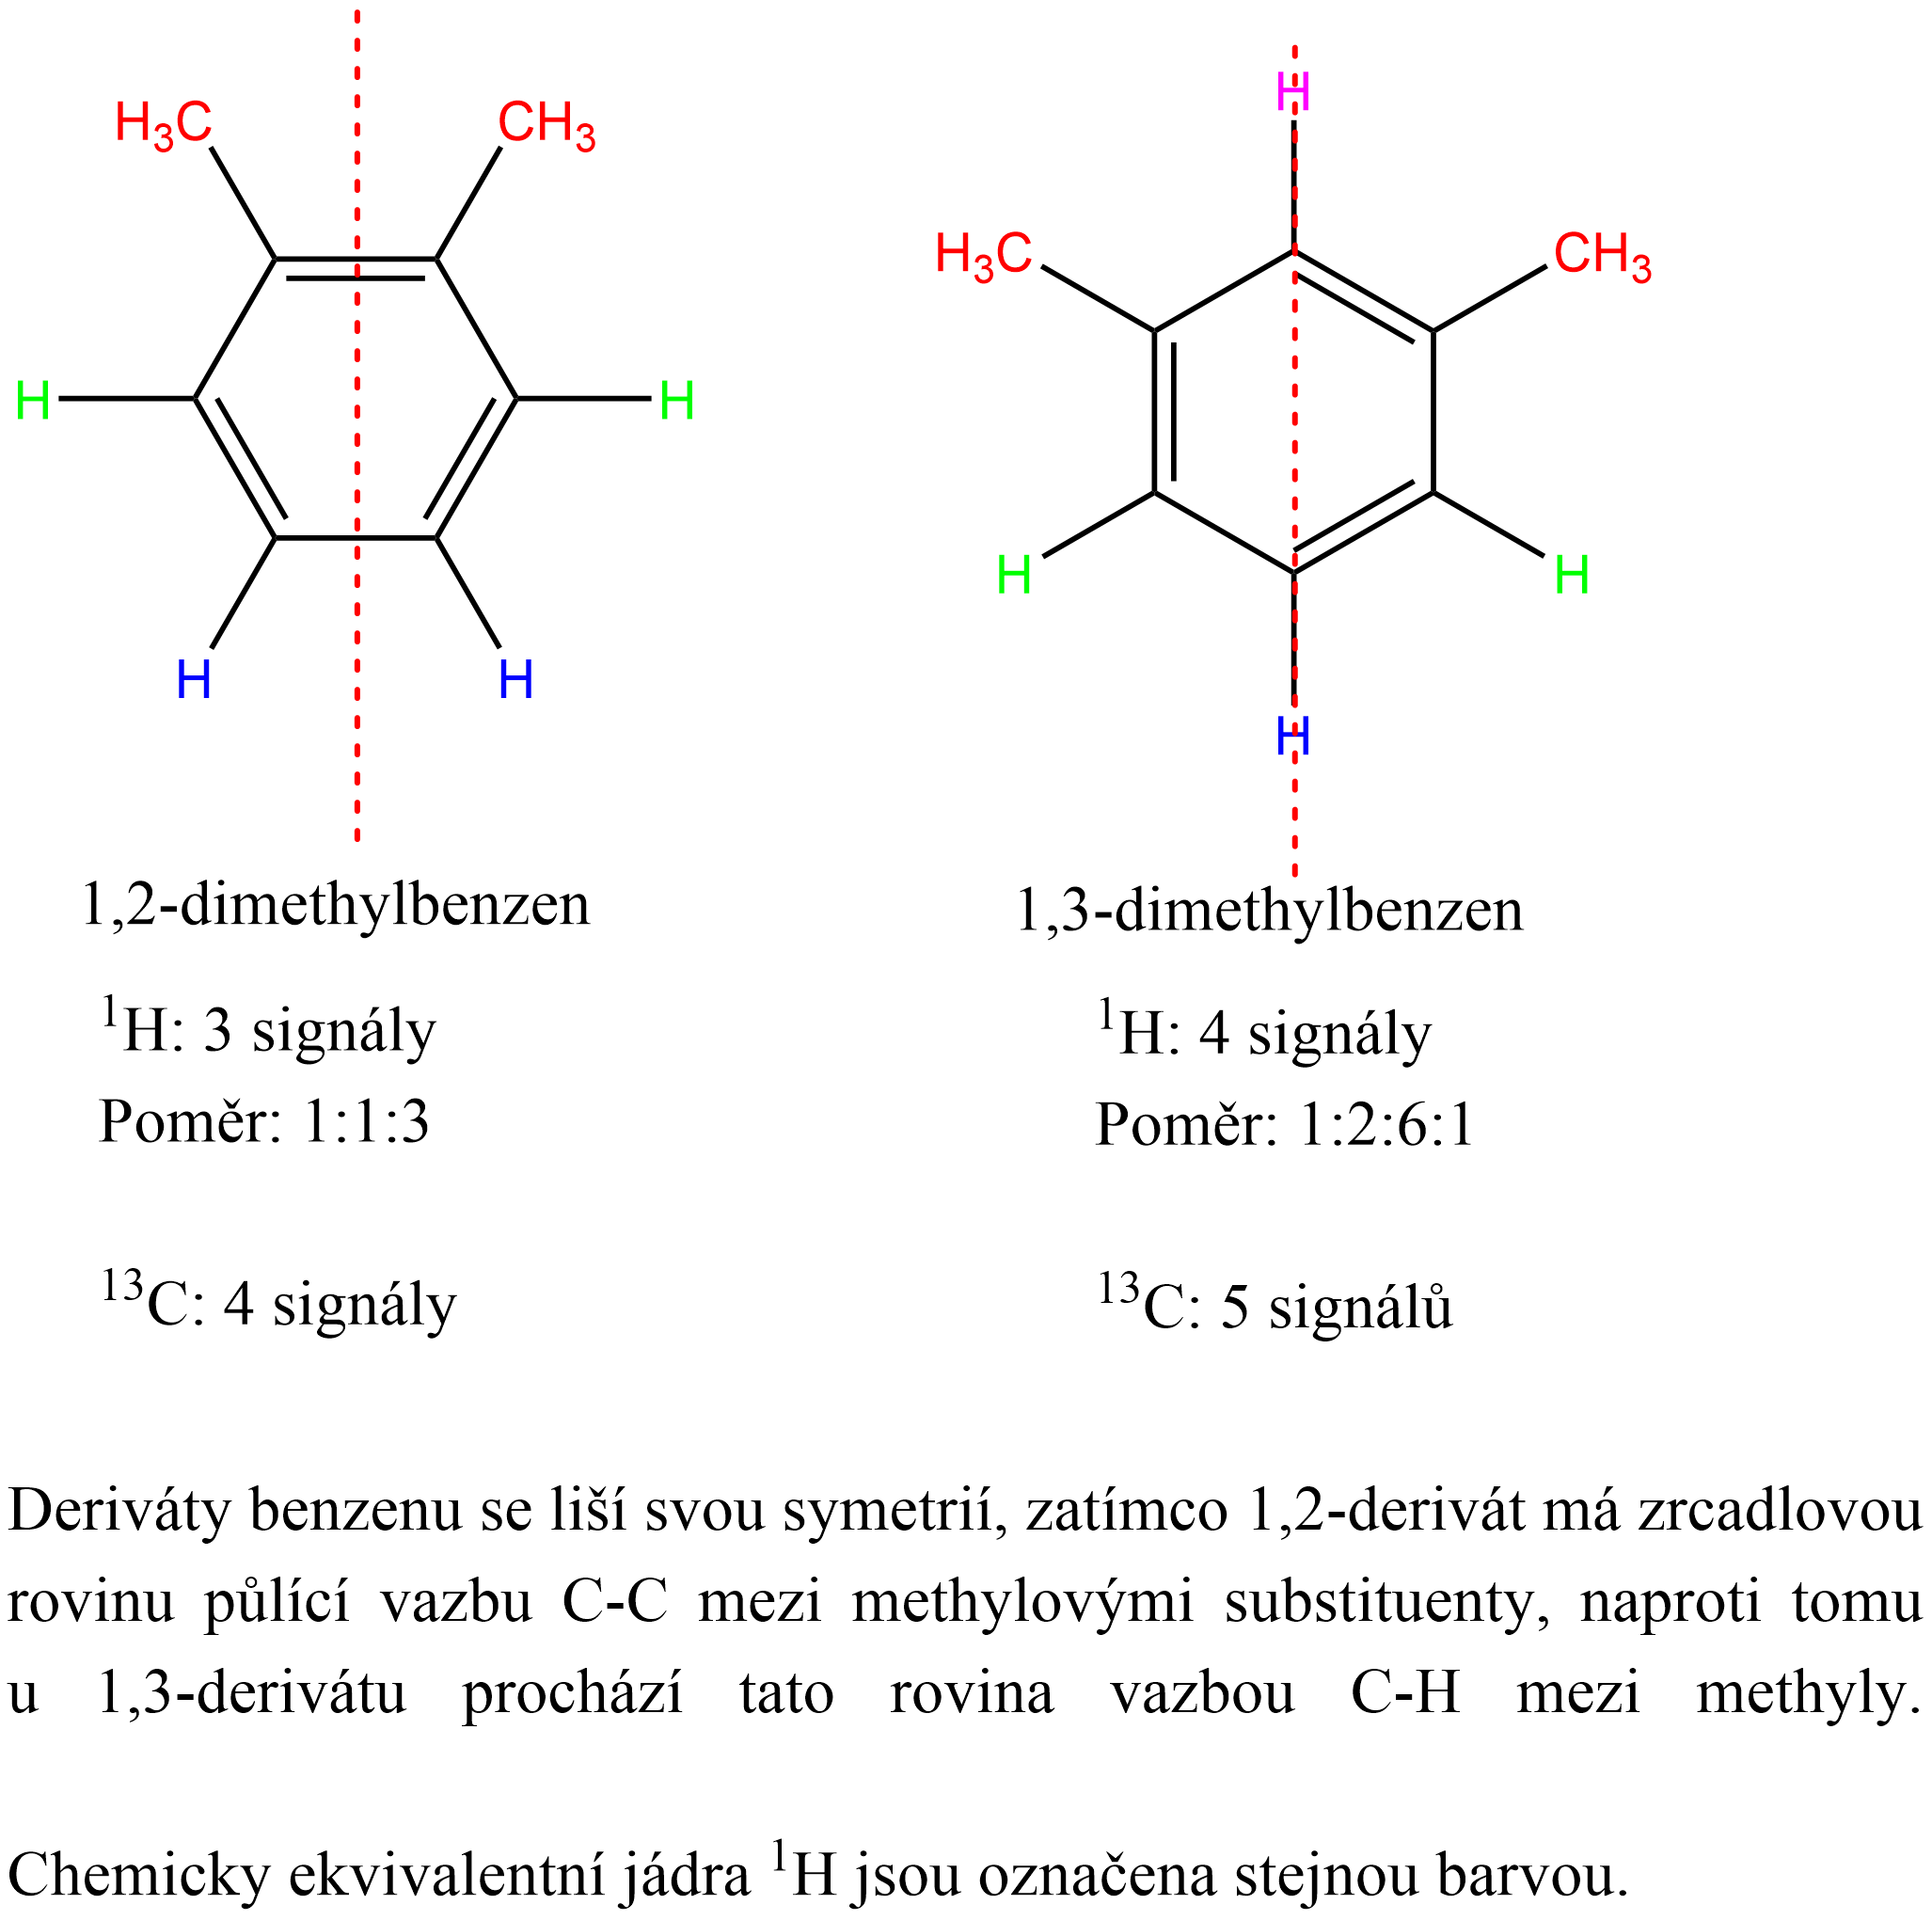
\includegraphics[width=.5\textwidth]{img/NMR1.png}

\begin{figure}[h]
	\adjincludegraphics[width=.3\textwidth]{img/NMR2.png}
\end{figure}

\begin{figure}[h]
	\adjincludegraphics[width=.3\textwidth]{img/NMR3.png}
\end{figure}